\documentclass{article}

\usepackage{color}
\usepackage[margin=1in]{geometry}
\usepackage{graphicx}
\usepackage{hyperref}
\usepackage{listings}

\definecolor{gray}{rgb}{0.5, 0.5, 0.5}
\definecolor{darkgreen}{rgb}{0, 0.6, 0}

\begin{document}
    \raggedright
    Homework 2 \break
    Christopher Seagraves
% % % % % % % % % % % % % % % % % % % % % % % % % % % % % % % % % % % % % % % % 

    \section*{Problem 1}
    \begin{minipage}{\linewidth}
        \raggedright
        ./Grid.py \break
        \url{https://github.com/nosv1/seagraves_unmanned_systems/blob/main/HW2/Grid.py}
        \lstset{
            frame=tb,
            language=Python,
            tabsize=4,
            numbers=left,
            basicstyle=\small\ttfamily,
            numberstyle=\tiny\color{gray},
            keywordstyle=\color{blue},
            commentstyle=\color{gray},
            stringstyle=\color{darkgreen}
        }
        \begin{lstlisting}
class Grid:

    ...

    def node_in_obstacle(self, position: Node) -> bool:
        """
        Checks if a position is in an obstacle
        :param position: position to check
        :return: True if in obstacle, False otherwise
        """
        for obstacle in self.obstacles:
            if position.distance(obstacle) <= self.obstacle_radius:
                return True
        return False
        \end{lstlisting}
    \end{minipage}
    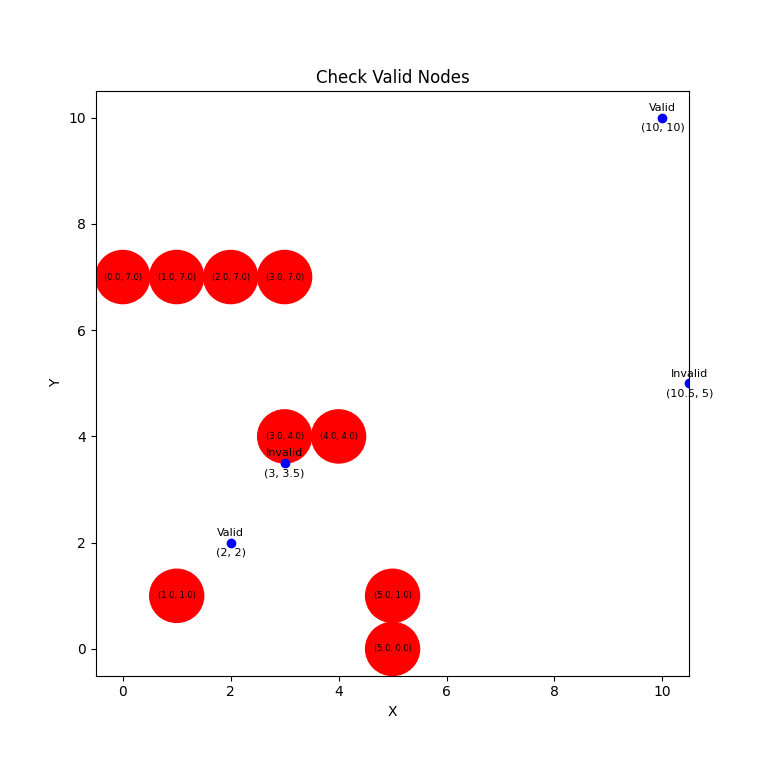
\includegraphics[height=3in]{HW2P1 Valid Positions.png}
% % % % % % % % % % % % % % % % % % % % % % % % % % % % % % % % % % % % % % % % 

\end{document}